\documentclass[a4paper]{article}   % list options between brackets
\usepackage{CJK}
\usepackage{fullpage}
\usepackage{graphicx}
\usepackage{graphics}
\usepackage{tabularx}
\usepackage{listings}
\usepackage{rotating}
\usepackage{setspace}
\usepackage{amsmath}
\usepackage{caption}
\usepackage{xcolor}
\usepackage{cite}

\lstset{numbers=left, numberstyle=\small, frame=shadowbox,
xleftmargin=1em,xrightmargin=1em, aboveskip=1em, breaklines,
extendedchars=false, tabsize=4, basicstyle=\linespread{1.0}\ttfamily,
commentstyle=\ttfamily\normal\small, keywordstyle=\color{blue!70}
}

% type user-defined commands here

\begin{document}
\begin{CJK}{UTF8}{gbsn}
\begin{spacing}{1.2}

\title{High Performance Computing\\ Homework 4\\ Report}
\author{Peiyun Hu, 2010011297\\Tsinghua.hp@gmail.com\\ [1em]Department of Computer Science \& Technology, Tsinghua University}
\maketitle

\section{Environment}
\subsection{CPU}
Intel(R) Core(TM) i7-2630QM CPU @ 2.00GHz
cpu cores	: 4
processors	: 8
\subsection{Compiler}
g++ (Ubuntu/Linaro 4.6.1-9ubuntu3) 4.6.1
mpic++(actually g++)
\subsection{Makefile}
The command used in Makefile is presented below in Listing~\ref{lst:makefile}.
\begin{lstlisting}[language=C, label=lst:makefile, caption=Makefile Command]
Problem 1:
	mpic++ -O2 -o mpi_int mpi_int.cpp -lm -lrt
	g++ -O2 -o openmp_int openmp_int.cpp -lm -lrt -fopenmp

Problem 2:
	mpic++ -O2 -o static static.cpp -lm -lrt
	mpic++ -O2 -o guided guided.cpp -lm -lrt
	mpic++ -O2 -o dynamic dynamic.cpp -lm -lrt

Problem 3:
	mpic++ -O2 -o study study.cpp -lm -lrt
\end{lstlisting}
\subsection{Run}
\begin{lstlisting}[language=C, label=lst:makefile, caption=Makefile Command]
Problem 1:
	mpirun -n $procs_num $bin $a $b $trapezoid_num

Problem 2:
static:
	mpirun -n $procs_num $bin $mode $std_sleep
dynamic: 
	mpirun -n $procs_num $bin $mode $std_sleep $chunk_size
guided: 
	mpirun -n $procs_num $bin $mode $std_sleep $chunk_size $shrink_factor

Problem 3:
	mpirun -n $procs_num $bin $OutputFile $shreshold

\end{lstlisting}

\subsection{Number of Processes and Threads}
Varied numbers of processes and threads are taken in different situations, and will be specified in the corresponding section of each problem. 

\section{The Comparison between OpenMP and MPI}
\subsection{Description}
In this section, we will discuss different methods, OpenMP and MPI, to calculate an integral of sin(x). Actually, when more processors are needed, MPI would be the primal choice, for the limit of thread numbers in a single computer. \textbf{However, we could see that MPI is also advantageous when number of processors involved is rather small.}

\subsubsection{Experiment}
For easy comparison, the interval of integral is defined in [0, 1.570796327], and the integrand is defined sin(x). 

Firstly, implements in MPI and OpenMP are compared. By the way, I also tried another implements in OpenMP. The former one uses 'Section' in OpenMP, while the extra one is implemented by leveraging 'Reduction' primitive. All primitives used are shown in Listing~\ref{lst:prob1_methods}.

\begin{lstlisting}[language=C, label=lst:prob1_methods, caption=Different Implements of OpenMP]
For Reduction:
#pragma omp parallel for reduction(+:res)

Sections:
#pragma omp parallel sections
{
#pragma omp section
...
#pragma omp section
}
\end{lstlisting}
\subsection{Performance}
In accuracy, \textbf{each method got almost identical results, but different on $10^{-16}$ digit}.

As to performance, that of each method is presented below in Figure~\ref{fig:prob1_perf}.

\begin{figure}[htbp]
\centering
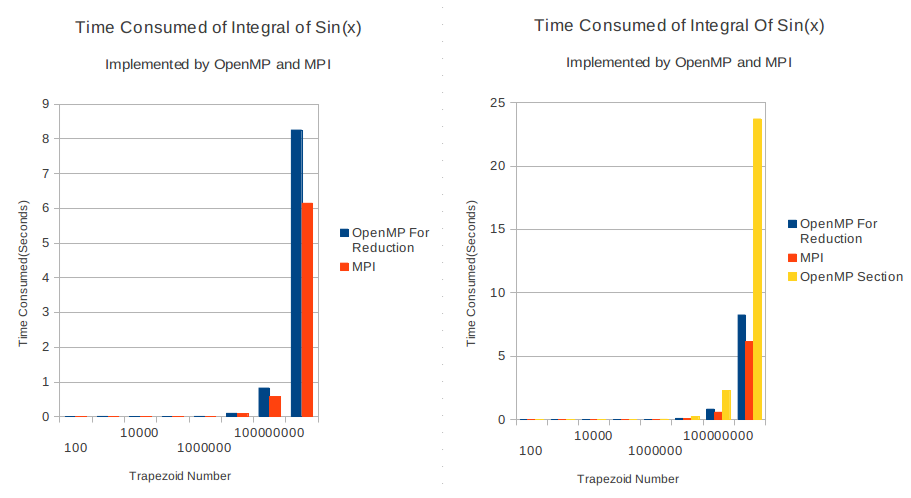
\includegraphics[width=12cm]{figs/prob1_Time.png}
\caption{Performance of Integral Using Different Methods}
\label{fig:prob1_perf}
\end{figure}
\textbf{MPI achieves a slightly better performance than OpenMP which uses 'Reduction'}, As we can see from above. 

\textbf{Another interesting thing is two different methods in OpenMP lead to totally different results.} However, the one using 'Section' achieves a rather poor performance as if it is not paralleled. After ensuring that it is programmed in parallel, I suppose that how the tasks are decomposed is critical to total performance, owing to the different workload of calculation of Sin(x) between different x, and Section is just not that fine in decomposition. 
\subsection{Conclusion}
\textbf{In Conclusion, we could achieve a better performance using MPI than OpenMP, when the number of processes and threads are identical.}

Though we achieve a better performance using MPI here, it owes to property of integral, in which no data must be shared and revised. If so, MPI would spare time to communication to synchronize. Moreover, in case there is data that must be shared and the workload is not enormously large, OpenMP is a rather good choice, indeed.

\section{Different Schedule Implemented in MPI}
\subsection{Description}
Different schedule implemented in MPI will be discussed in this section. Specifically, we implement 'Static', 'Dynamic' and 'Guided'. In detail, each process deals with the same workload when 'Static' schedule is taken, dynamically allocated chunks of certain size if 'Dynamic' is taken, and get chunks whose size shrink to certain amount every time allocated when 'Guided' is taken. 

\subsubsection{Experiment}
To show advantages of each kind of schedule, I design three 'Dummy' function respectively. 
\begin{align}
\text{Dummy 1}: std\_sleep*1.5
\end{align}
\begin{align}
\text{Dummy 2}: std\_sleep*(1+task\_id/task\_num)
\end{align}
\begin{align}
\text{Dummy 3}: std\_sleep*(sin(2*PI*task\_id/task\_num) + 1.5)
\end{align}

The 3 different functions have the same average, however, have different ways of changing. The figure of Schedule Function is presented below in Figure ~\ref{fig:prob2_schedule}.

\begin{figure}[htbp]
\centering
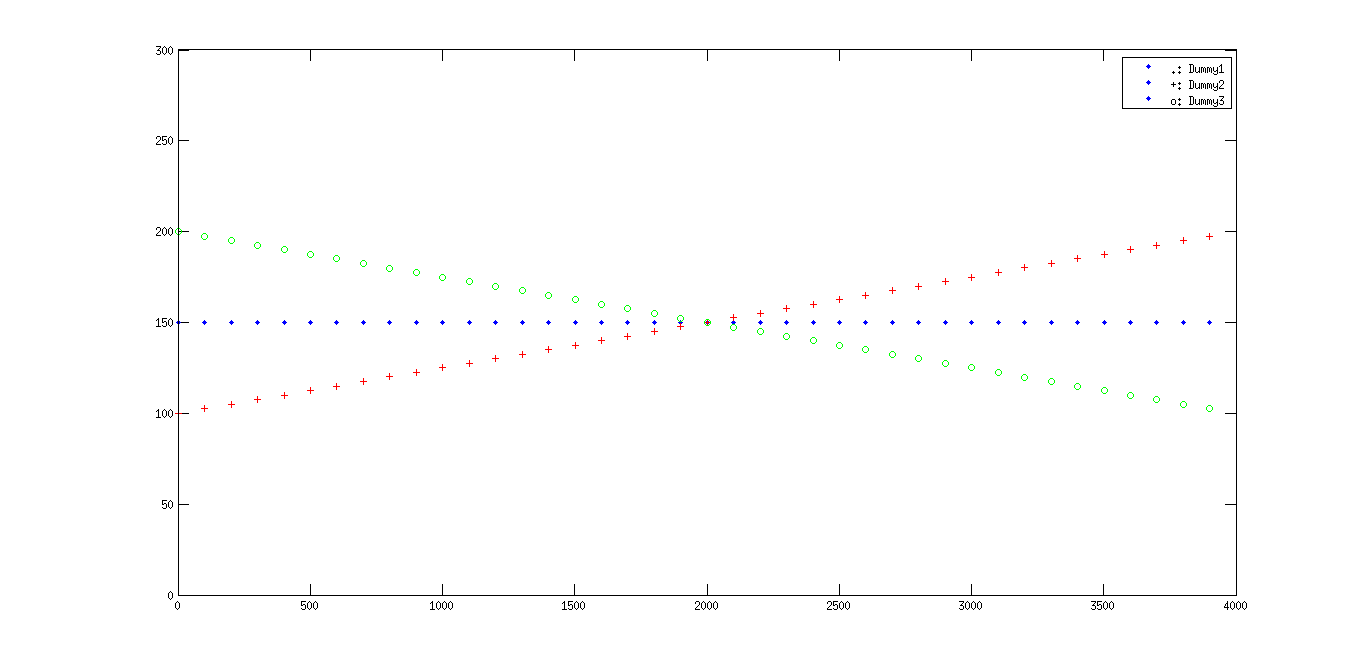
\includegraphics[width=12cm]{figs/prob2_schedule.png}
\caption{Figures of the Three Dummy Function}
\label{fig:prob2_schedule}
\end{figure}

In addition, I assign the chunk size 100 for both 'Dynamic' and 'Guided' schedule for easy comparison. The exponential of shrink of chunk size is assigned 1.1505, which comes from tests.

What should be noted is that there is a master process in the implement of 'Dynamic' Schedule. Owing to the upper bound of number of processes and reasonable comparison, \textbf{we limit the process number of 'Static' Schedule and 'Guided' Schedule to 3}. And there is a master process which did nothing but send and receive and 3 slaves processes which call dummy function in 'Dynamic' Schedule. For we expect to find the advantages and disadvantages of different methods of allocation, the restriction makes sense.

\subsection{Performance}
The performance of three schedules as to three Dummy Functions is presented below in Figure~\ref{fig:prob2_performance}.
\begin{figure}[htbp]
\centering
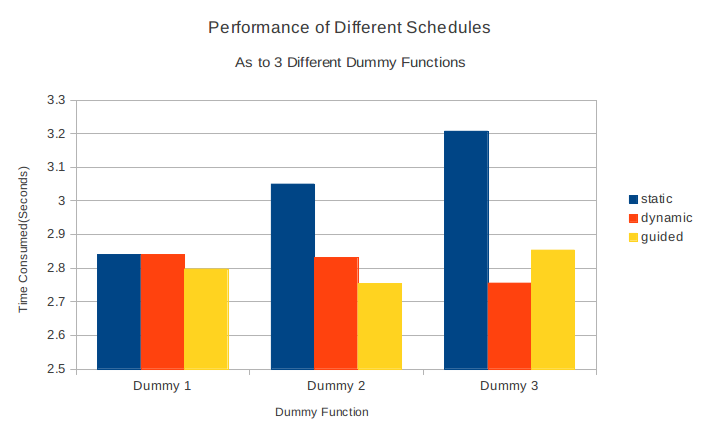
\includegraphics[width=12cm]{figs/prob2_performance.png}
\caption{Performance}
\label{fig:prob2_performance}
\end{figure}

As is shown in the Figure~\ref{fig:prob2_performance}, we could find that 'Dynamic' always achieve a decent performance, and so is guided, however, the 'Static' Schedule is quite sensitive on the distribution of workload, and reach poor performance when the workload distribution is complex. 

In Dummy 1, 'Static', 'Dynamic' and 'Guided' all achieve a rather good performance. While, in Dummy 2, the time consumed using 'Static' increases sharply, but the other two stay the same. Actually, 'Guided' schedule is advantageous in this distribution of workload, for the shrink of chunk size could balance the influence of increasing workload of each task. Besides, 'Dynamic' is also adaptable in all kinds of complex distribution of workload. However, when considering Dummy 3, there are minute difference between 'Guided' and 'Dynamic' that, specifically, slight unbalance would arise at very beginning when each task has a rather larger overhead as to 'Guided', on the other hand, 'Dynamic' could adapt to this owing to its flexibility. 
\subsection{Conclusion}
\textbf{In Conclusion, both guided and dynamic are adaptable in complex distribution of workload, besides, static is less adaptive. } While, as to 'Dynamic' schedule(specially in MPI), there is overhead of communication and there would be a process spared to be the master process. On the other hand, though 'Guided' would cause unbalance under some extreme conditions, it is rather a good schedule for its simplicity, lower communication overhead, and no master process. What is more, 'Static' is the most common schedule we choose for simple use, especially when tasks are on the same level of overhead, but it should be replaced by other schedules when distribution is changing apparently, in consideration of performance. 

\section{Study Night}
\subsection{Description}
See the detailed description of Study Night in the homework handout. The central point at this issue is how we dispatch tasks when the performance of each processor is not on the same level. In this problem, students are not the averagely skilled in solving exercises. And we should find them a schedule which make sure the total time is as short as possible. 

\subsection{Implement}
For general purpose, I did not try to implement it with some static strategy, but find a rather universal and convenient schedule to handle the dispatching problem. And a trick is used to optimize performance, which is not thtat universal. 

There are 5 processes created to handle this, of which one is a master process, the other 4 are slave processes. For that the time spent in solving problems is certain, we could foresee the next time when slave process will be idle again, and in this way, the master process could choose whether or when to send tasks to slave processes by itself. 

Besides, all processes have simultaneous clock, which is implemented by using 'MPI\_Barrier()'. And nothing will be done actually in slave processes, All slave process should do is receive tasks and decide whether break out of the dead loop. While, the master process would send tasks to certain slave processes and record the next time the slave process will be idle. Everytime the time is changed, it will be compared with the next idle time of each slave process. Once equal, the master process will send task out, and overwrite the next idle time. Additionally, which task to send is determined in the getTask(), the more skilled will do harder exercises, the less skilled is tended to do easier exercises and more verification. 

More specifically, a task pool is updated in order to make sure that it would be sorted well everytime changed. We define the relationship between processes' level of skills like~(\ref{align:prob2_skill}).
\begin{align}\label{align:prob2_skill}
P1 < P2 < P3 < P4
\end{align}
P1 will be always sent the least time-cost thing, no matter verification or solution. What P2 will be rendered is exercises whose time consumed is in about $\frac{1}{3}$ of the task pool. P3 is almost similar with P2, but $\frac{2}{3}$ of the sequence. Finally, P4 will always do the most tough work in the task pool.

By the way, a small trick is taken to optimize the performance. In detail, tasks will cost P1 or P2 more than 1000 seconds are not allowed to be sent to those two processes after 3800 seconds. And this trick achieve a decline of about 700 seconds in total time. 
\subsection{Performance}
The results of allocation is presented in Figure~\ref{fig:prob3_solution} and Figure~\ref{fig:prob3_verification}. 
\begin{figure}[htbp]
\centering
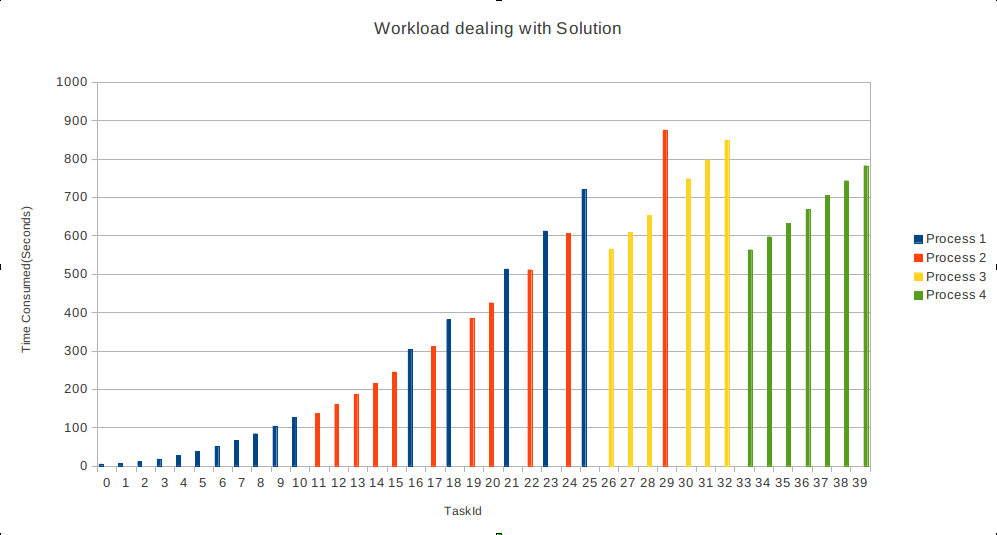
\includegraphics[width=12cm]{figs/prob3_SolutionDistribution.png}
\caption{The Result of Solution Allocation}
\label{fig:prob3_solution}
\end{figure}

\begin{figure}[htbp]
\centering
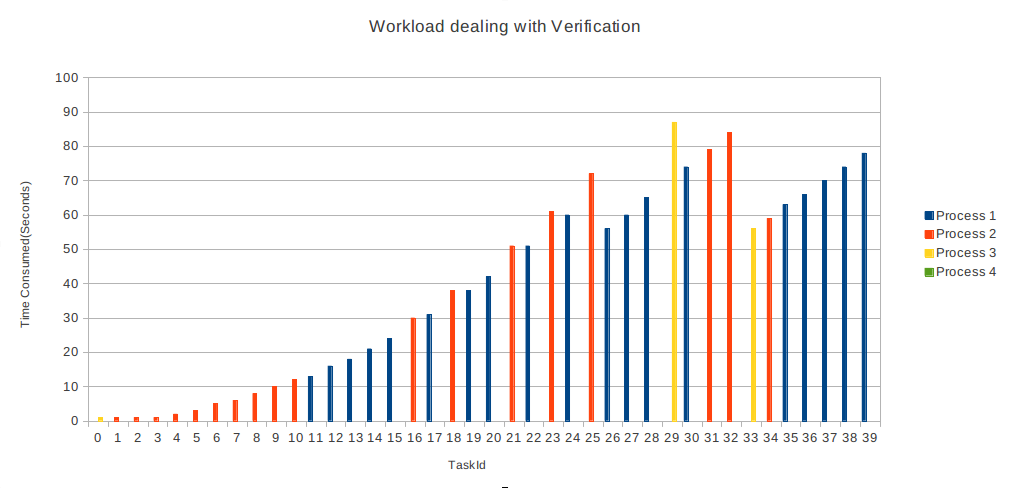
\includegraphics[width=12cm]{figs/prob3_VerificationDistribution.png}
\caption{The Result of Verification Allocation}
\label{fig:prob3_verification}
\end{figure}

As we could see from Figure~\ref{fig:prob3_solution}, it seems like less skilled processes handled easier exercises, and more skilled ones handled tougher exercises. And in Figure~\ref{fig:prob3_verification}, we could see that P1 do most work of the verification, then P2, P3. P4 has never verify any exercises, which is ideal, as well.

Moreover, the total workload of each process is presented in Table~1.

\begin{table}[htbp]
\label{tab:prob3_workload}
\centering
\begin{tabular}{|c|c|c|c|c|}
\hline • & Process 1 & Process 2 & Process 3 & Process 4 \\ 
\hline Solution(Seconds) & 3069 & 4057 & 4219 & 4690 \\ 
\hline Verification(Seconds) & 920 & 523 & 144 & 4690 \\ 
\hline Total(Seconds) & 3989 & 4580 & 4363 & 4690 \\ 
\hline 
\end{tabular} 
\caption{The Total Workload of Each Process}
\end{table}

Noting that the total time is 4691, we could see that the most capable process almost never stops working, and those less skilled processes do a rather balanced job, indeed. 

\subsection{Conclusion}
\textbf{In Conclusion, to dispatch tasks in order of the capability of processes is a good way to balance workload and optimize the total execution time.} On this basis, we could more easily use some targeted tricks to improve. For example, in Figure~\ref{fig:prob2_performance}, we could see that P2 took the longest time to solve a problem. With some more restrictions, there could be some tasks exchange between P2 and P3, and higher performance would probably be reached. However, what we focus on is a rather universal method to solve problems of this kind, overmuch tricks would not make more sense.


\bibliographystyle{plain}
\bibliography{bibitex}

\appendix
\section*{Appendix}
\section{Code Package}
\subsection{Directories}
./code:
problem1  problem2  problem3

./code/problem1:
mpi\_int.cpp openmp\_int.cpp

./code/problem2:
static.cpp dynamic.cpp guided.cpp

./code/problem3:
study.cpp
\section{OutputFile of Problem 3}
\begin{lstlisting}
Total Study Time:4691
Format: (startTime, timeSustained, processId, taskId, (verification or solution))
(0, 5, 1, 0, s)
(0, 187, 2, 13, s)
(0, 565, 3, 26, s)
(0, 782, 4, 39, s)
(5, 7, 1, 1, s)
(12, 12, 1, 2, s)
(24, 18, 1, 3, s)
(42, 18, 1, 13, v)
(60, 27, 1, 4, s)
(87, 38, 1, 5, s)
(125, 51, 1, 6, s)
(176, 56, 1, 26, v)
(187, 137, 2, 11, s)
(232, 13, 1, 11, v)
(245, 67, 1, 7, s)
(312, 84, 1, 8, s)
(324, 161, 2, 12, s)
(396, 16, 1, 12, v)
(412, 78, 1, 39, v)
(485, 215, 2, 14, s)
(490, 21, 1, 14, v)
(511, 104, 1, 9, s)
(565, 608, 3, 27, s)
(615, 60, 1, 27, v)
(675, 126, 1, 10, s)
(700, 245, 2, 15, s)
(782, 743, 4, 38, s)
(801, 24, 1, 15, v)
(825, 74, 1, 38, v)
(899, 304, 1, 16, s)
(945, 12, 2, 10, v)
(957, 30, 2, 16, v)
(987, 10, 2, 9, v)
(997, 311, 2, 17, s)
(1173, 653, 3, 28, s)
(1203, 31, 1, 17, v)
(1234, 65, 1, 28, v)
(1299, 381, 1, 18, s)
(1308, 8, 2, 8, v)
(1316, 38, 2, 18, v)
(1354, 385, 2, 19, s)
(1525, 705, 4, 37, s)
(1680, 38, 1, 19, v)
(1718, 70, 1, 37, v)
(1739, 6, 2, 7, v)
(1745, 425, 2, 20, s)
(1788, 42, 1, 20, v)
(1826, 748, 3, 30, s)
(1830, 74, 1, 30, v)
(1904, 513, 1, 21, s)
(2170, 5, 2, 6, v)
(2175, 51, 2, 21, v)
(2226, 3, 2, 5, v)
(2229, 511, 2, 22, s)
(2230, 668, 4, 36, s)
(2417, 51, 1, 22, v)
(2468, 66, 1, 36, v)
(2534, 612, 1, 23, s)
(2574, 797, 3, 31, s)
(2740, 2, 2, 4, v)
(2742, 61, 2, 23, v)
(2803, 79, 2, 31, v)
(2882, 1, 2, 3, v)
(2883, 605, 2, 24, s)
(2898, 632, 4, 35, s)
(3146, 60, 1, 24, v)
(3206, 63, 1, 35, v)
(3269, 720, 1, 25, s)
(3371, 848, 3, 32, s)
(3488, 1, 2, 2, v)
(3489, 72, 2, 25, v)
(3530, 597, 4, 34, s)
(3561, 59, 2, 34, v)
(3620, 0, 2, 1, v)
(3621, 84, 2, 32, v)
(3705, 875, 2, 29, s)
(4127, 563, 4, 33, s)
(4219, 56, 3, 33, v)
(4275, 87, 3, 29, v)
(4362, 0, 3, 0, v)
Process 1
(0, s) (1, s) (2, s) (3, s) (13, v) (4, s) (5, s) (6, s) (26, v) (11, v) (7, s) (8, s) (12, v) (39, v) (14, v) (9, s) (27, v) (10, s) (15, v) (38, v) (16, s) (17, v) (28, v) (18, s) (19, v) (37, v) (20, v) (30, v) (21, s) (22, v) (36, v) (23, s) (24, v) (35, v) (25, s) 
Process 2
(13, s) (11, s) (12, s) (14, s) (15, s) (10, v) (16, v) (9, v) (17, s) (8, v) (18, v) (19, s) (7, v) (20, s) (6, v) (21, v) (5, v) (22, s) (4, v) (23, v) (31, v) (3, v) (24, s) (2, v) (25, v) (34, v) (1, v) (32, v) (29, s) 
Process 3
(26, s) (27, s) (28, s) (30, s) (31, s) (32, s) (33, v) (29, v) (0, v) 
Process 4
(39, s) (38, s) (37, s) (36, s) (35, s) (34, s) (33, s) 

\end{lstlisting}

\end{spacing}
\end{CJK}
\end{document}
